\documentclass[11pt,letterpaper]{article}

% include figures
\usepackage{graphicx}
% get nice colors
\usepackage{xcolor}

% change default font to Palatino (looks nicer!)
\usepackage[latin1]{inputenc}
\usepackage{mathpazo}
\usepackage[T1]{fontenc}
% load some useful math symbols/fonts
\usepackage{latexsym,amsfonts,amsmath,amssymb,wasysym}
% be able to insert code
\usepackage{listings}

% comfort package to easily set margins
\usepackage[top=1in, bottom=1in, left=1in, right=1in]{geometry}

% spacing after a paragraph
\setlength{\parskip}{.15cm}
% indentation at the top of a new paragraph
\setlength{\parindent}{0.0cm}
% make units not slanted in math mode
\newcommand{\unit}[1]{\ensuremath{\, \mathrm{#1}}}

\begin{document}

\begin{center}
\Large
Ay190 -- Worksheet 13\\
Daniel DeFelippis\\
Date: \today
\end{center}

%%
%%
%% I worked with Scott Barenfeld
%%
%% All python code can be found in the ws13 directory in my repository
%%
%%

\section*{Direct Summation N-Body Code}


We are solving an N-body gravitational system:
$$ \mathbf{\ddot{x}}_i = -G\sum\limits_{j=1,i \neq j}^{N} \frac{m_j}{|\mathbf{x}_{ij}|^2} \mathbf{\hat{x}}_{ij}$$
using direct summation code. The data file has six rows: three coordinates (xyz) and three 
velocities (xyz). I edited the code skeleton to create a function which 
computes the right hand side (RHS) of the resulting three equations for each object, 
as well as an RK4 integrator. 

\section{}

By running the code for the Sun-Earth system, we confirm that
the code works: the Earth rotates the Sun at a visually constant radius over a year. 
However, if the step size is too small, going for multiple years results in the Earth 
spiraling inwards and being flung out of orbit fairly quickly. To see why this happens, I 
wrote a function which computes the total energy of the N-body system given by 
$$ E_{tot} = \sum\limits_{i=1}^N \frac{1}{2} m_i |\mathbf{v}_i|^2 
             -G\sum\limits_{i,j=1,i\neq k}^N \frac{m_i m_j}{|\mathbf{x}_{ij}|}. $$ 
Graphing the total energy over time with different values of the number of steps, we see
that the energy doesn't necessarily remain constant. Sometimes it spikes up to a very
large positive value, corresponding to the Earth being flung out of orbit. Even when that
doesn't happen though, for larger numbers of time steps, the total energy oscillates, as
shown by the green line in figure~\ref{fig:sunearth}. Energy doesn't remain constant here 
probably because the orbit is discretized compared to what actually happens, causing 
small errors in the location of the Earth and therefore errors in the energy. 

\begin{figure}[bth]
\centering
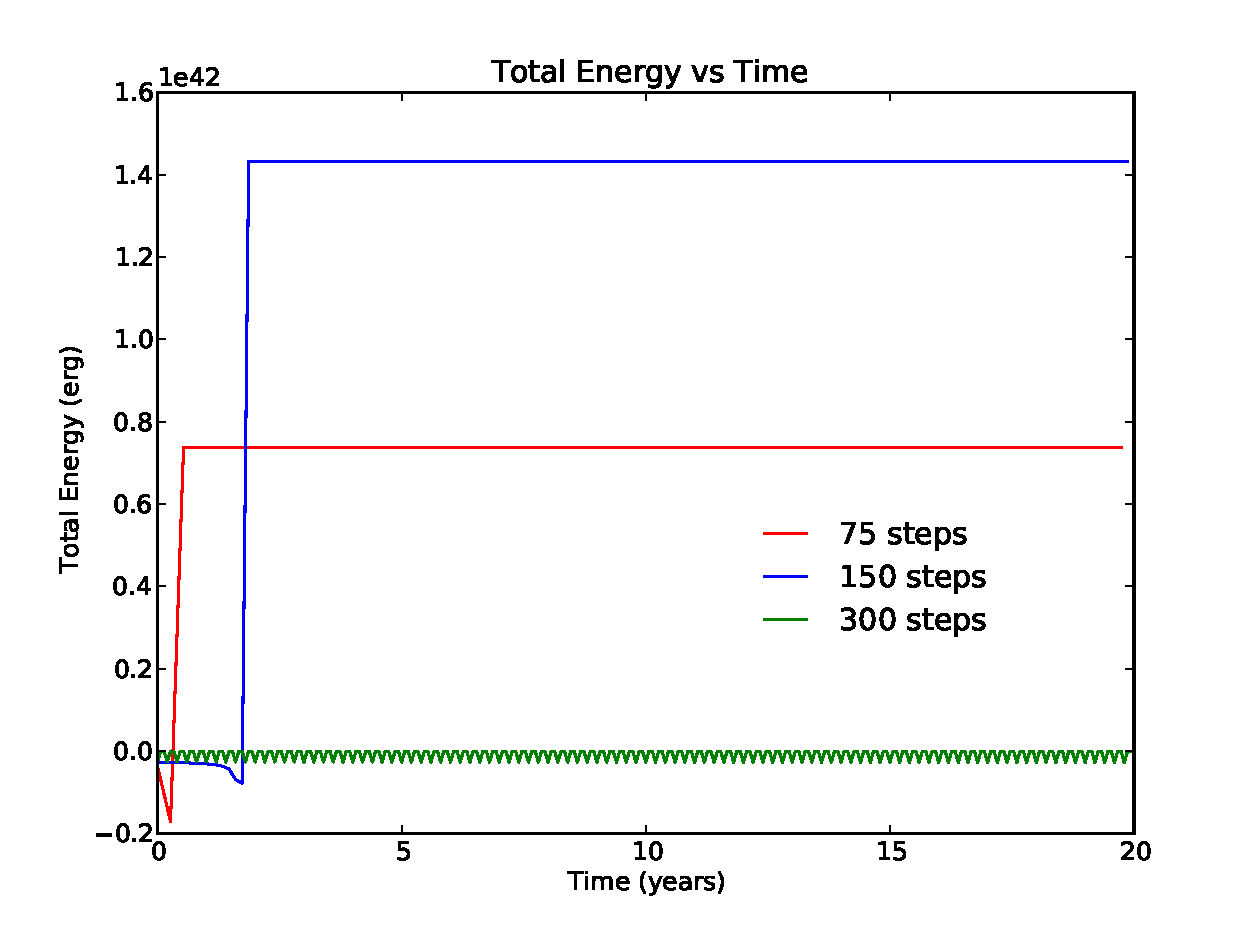
\includegraphics[width=\textwidth]{energy.pdf}
\caption{Plot of Total Energy vs time for Sun-Earth system}
\label{fig:sunearth}
\end{figure}



\section{}

Next, we use our code on a more complicated system, a 13-star system orbiting a black hole.
If I used too many steps, the code became unbearably slow, so I limited myself to 200 
steps over 10 years. If we plot the energy here, we again see that the stars are flung 
out of orbit even more quickly than in the Sun-Earth system, as shown in
figure~\ref{fig:stars}. They didn't all get flung out at the same time: the horizontal 
sections correspond to a particular star maintaining an "orbit" for a short period
of time longer than the rest of the stars.

\begin{figure}[bth]
\centering
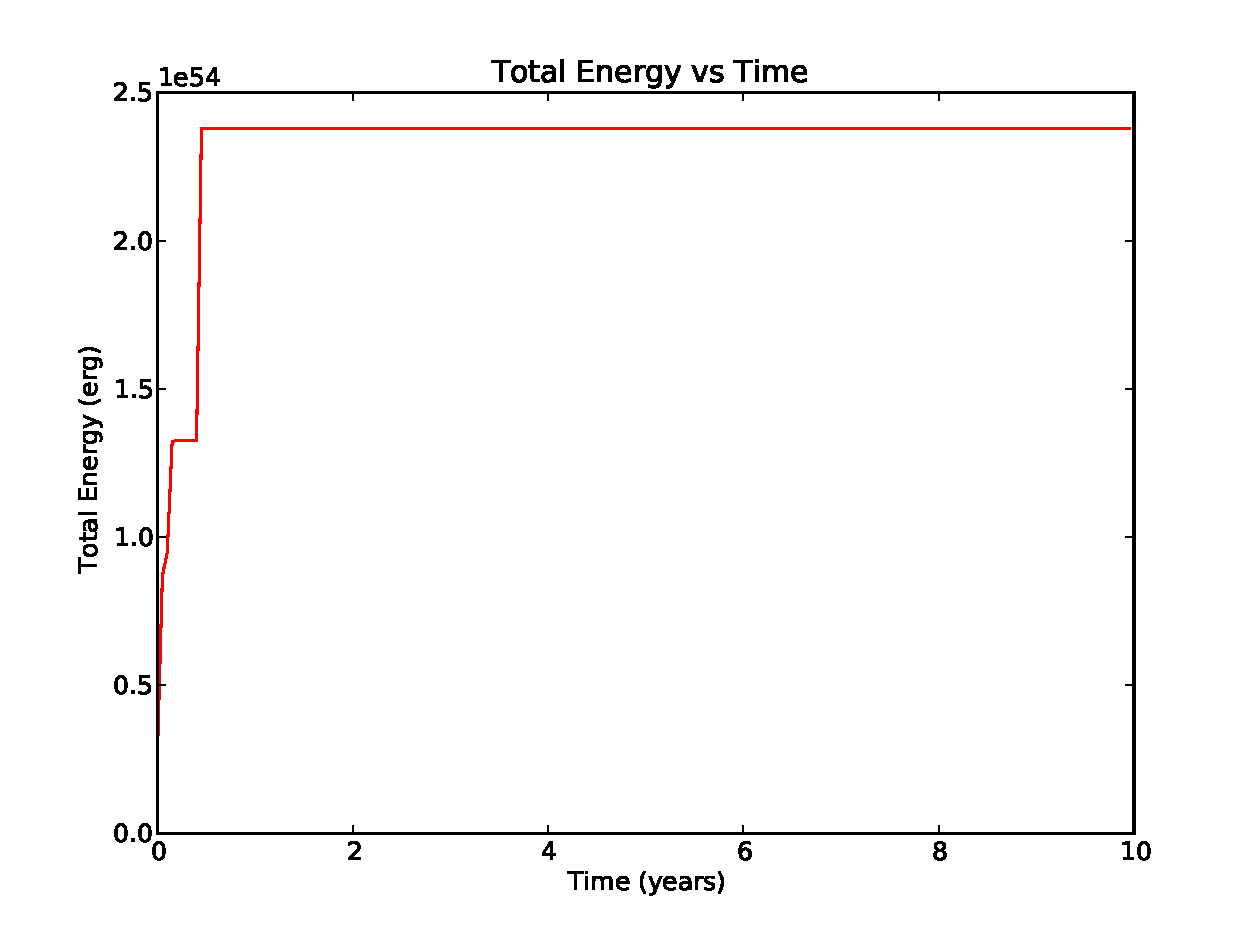
\includegraphics[width=\textwidth]{energy_stars.pdf}
\caption{Plot of Total Energy vs time for 13 Stars and Black Hole}
\label{fig:stars}
\end{figure}

Getting rid of the unit conversions so we can just watch the stars evolve on a scale of 
arcseconds, we see that they quickly exceed the maximum initial value of each coordinate 
very quickly, contrary to the actual data from the data file from the uchicago website. 
In that actual data, the stars never have a coordinate with a larger magnitude than 3 
arcseconds. My code however places the stars very much outside that range quickly, which
can be seen by increasing value of "rmax" on the 3D plot and watching the stars 
\textit{still} exceed the axes. So, as expected, this basic method of evolving N-body
systems does not work very well for even $N=14$.

\end{document}
